\documentclass[11pt]{article}
\usepackage[paperwidth=12cm, paperheight=18cm, margin=1cm]{geometry}
\usepackage{amsmath, tikz}
\pagestyle{empty}

\begin{document}
\begin{center}
  {\LARGE\bfseries The Base Rate Fallacy}\\[4pt]
  {\large A 99\% accurate test, and you're probably fine}
\end{center}

A disease affects 1 in 1000 people. A test catches 99\% of
sick people and wrongly flags 1\% of healthy ones.
You test positive. Are you sick?

\section*{Bayes' theorem}
\[
  P(S \mid +) = \frac{P(+ \mid S)\,P(S)}
    {P(+ \mid S)\,P(S) + P(+ \mid H)\,P(H)}
\]
\[
  P(S \mid +) = \frac{0.99 \cdot 0.001}
    {0.99 \cdot 0.001 + 0.01 \cdot 0.999} \approx 9\%
\]

\section*{Count people instead}
\begin{center}
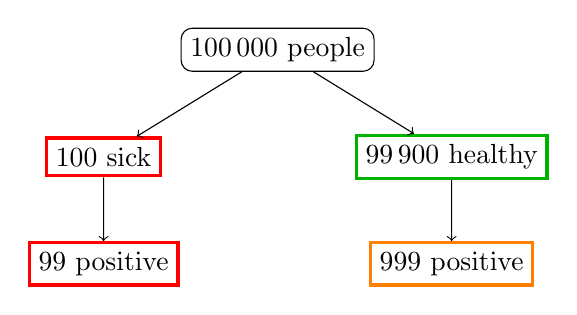
\begin{tikzpicture}[scale=0.85]
  \node[draw, rounded corners] (all) at (0,0) {100\,000 people};
  \node[draw=red, very thick] (sick) at (-2.6,-1.6) {100 sick};
  \node[draw=green!70!black, very thick] (ok) at (2.6,-1.6) {99\,900 healthy};
  \node[draw=red, very thick] (tp) at (-2.6,-3.2) {99 positive};
  \node[draw=orange, very thick] (fp) at (2.6,-3.2) {999 positive};
  \draw[->] (all) -- (sick);
  \draw[->] (all) -- (ok);
  \draw[->] (sick) -- (tp);
  \draw[->] (ok) -- (fp);
\end{tikzpicture}
\end{center}
\[
  \frac{99}{99 + 999} = \frac{99}{1098} \approx 9\%
\]
\centerline{\bfseries Rare diseases make false alarms the majority.}
\end{document}
